\subsubsection{Biological Effects of Electromagnetic Radiation}
\index{Lerchl, Alexander}

\paragraph{Research Team}
Alexander Lerchl (Professor), Karen Grote (Lab Assistant), Melanie Klose (PhD Student), Kirsten Schwarzpaul (Research Associate), Tatjana Simon (Lab Technician), Angela Sommer (Research Associate), Thomas Str�hlein (Animal Keeper) \\

The research interests of our group covers a range of topics which are related to the effects of visible light and non-visible electromagnetic radiation on animals and humans. Biological parameters investigated are from direct actions of light with photopigments, effects on the biological clock, induction of cancer, and survival analysis. The methods include immunocytochemistry, \textit{in vitro} and \textit{in vivo} experiments, and statistical analyses of large-scale population data sets. The overall goal is to determine how natural and anthropogenic physical stimuli from the environment can influence life.


\paragraph{Highlights}
%
Possible adverse health affects of nonvisible electromagnetic
radiation, e.g., originating from mobile phones, are a great concern
for the general public and the political decision makers. Although
these non-thermal, non-ionizing fields are too low in energy to
cause direct effects on molecules (unlike ionizing radiation), there
is a strong need for studies addressing this issue. Ideally, these
studies should be completed before a new generation of mobile phones
is introduced. Supported by the government the team has performed a
series of experiments involving special mice which spontaneously
develop lymphoma. These experiments were performed both with
magnetic fields of various intensities (1, 100, and 1000
$\mu$Tesla), and frequencies of the GSM (900 MHz) and new UMTS
standard (approx. 1900 MHz). So far, no adverse effects were
observed. A new experiment with normal mice is currently being
performed, this time looking for teratogenic effects in animals
which are continuously exposed over three generations (Fig.
~\ref{fig:proflerchl}). The study will be finished in 2007.

\begin{figure}[ht]
\begin{center}
   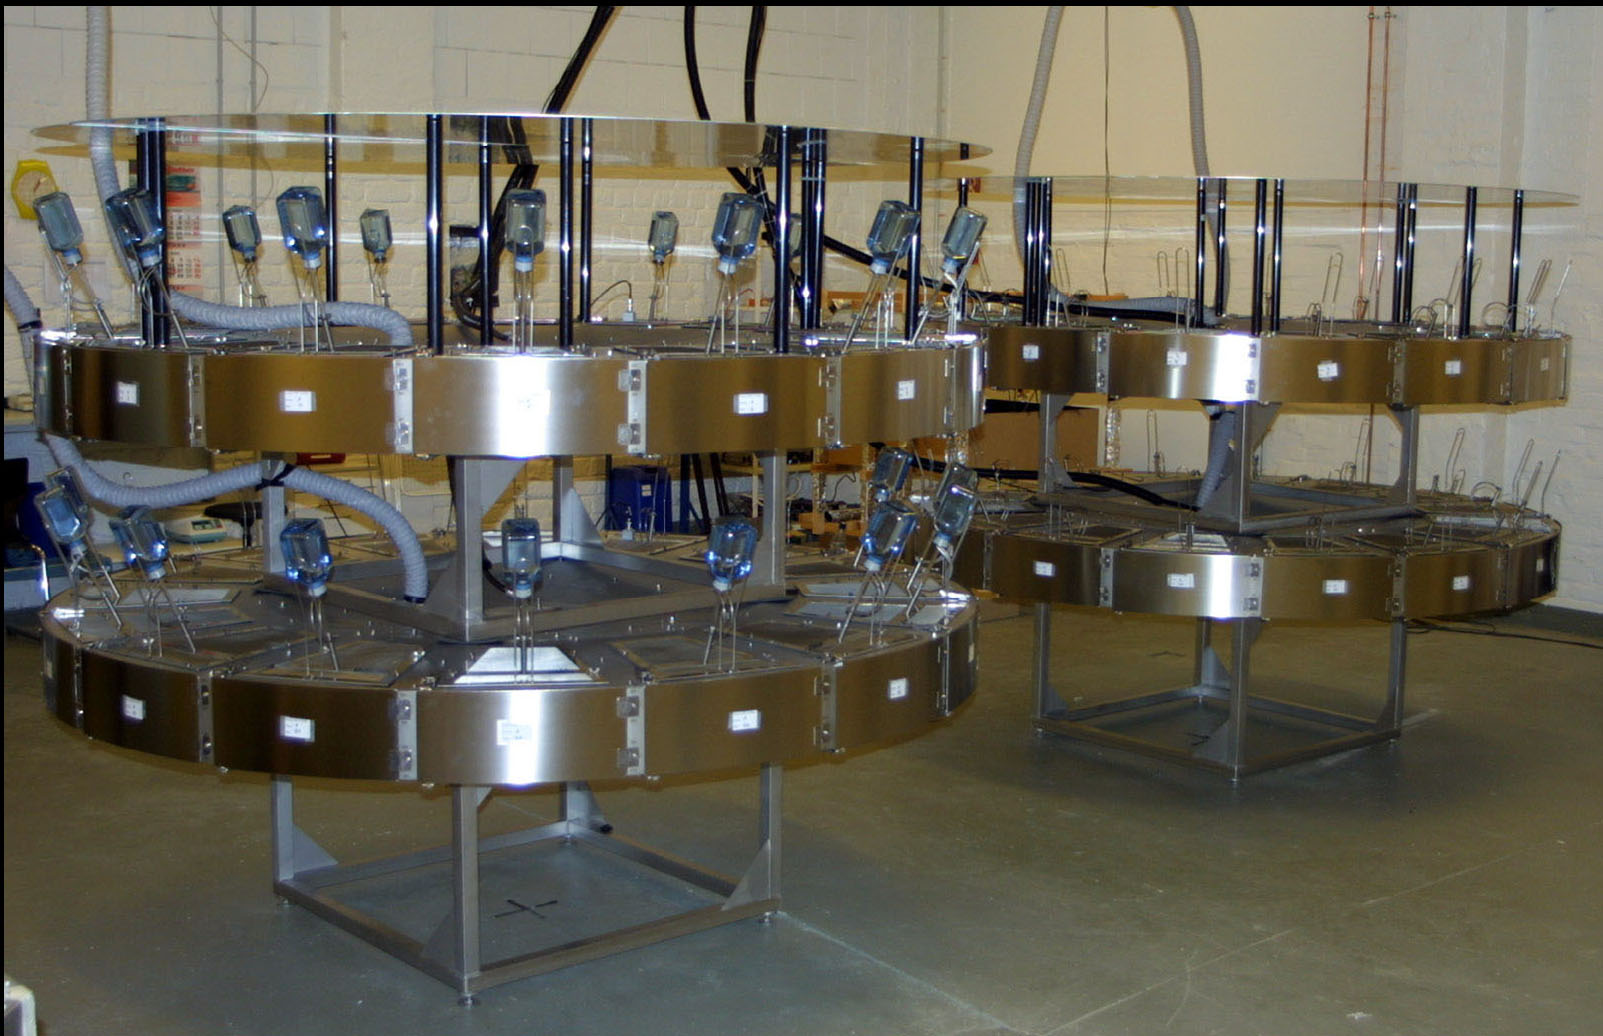
\includegraphics[width=\hsize]{Lerchl/proflerchl-fig1.jpg}
\mycaption{ Two of four exposure units for the long-term study in normal mice.
In each unit, 32 breeding pairs are continuously exposed to electromagnetic fields at exposure doses relevant to humans. }
\label{fig:proflerchl}
\end{center}
\end{figure}

A recent publication by the Robert-Koch Institute, the German governmental agency for public health issues, with Professor Lerchl as external expert, classifies blood tests in humans as not suited for detecting adverse effects of radiation by mobile phone base stations.

Another area of research in Djungarian hamsters (\textit{Phodopus sungorus}) revealed that Sertoli cells, contradicting a previous dogma, are not terminally differentiated, but can be stimulated by Follicle Stimulating Hormone. These cells, important for the production of testicular sperm, are thus able to enter a transitional stage exhibiting features of both differentiated and undifferentiated Sertoli cells. These results are of potential clinical relevance for subfertile or infertile men with idiopathic (unexplained) low sperm counts.




\myparagraph{Collaborations}
Bremen Area Collaborations:
\begin{enumerate}
\item {\sl International University Bremen} \\ Prof. A. Materny \\ Raman spectroscopy of normal and cancer tissues
  \\ Prof. V.B. Meyer-Rochow \\ Theoretical work on evolution of visual pigments
\end{enumerate}
National \& International Collaborations:
\begin{enumerate}
\item {\sl Monash University, Australia} \\ Dr. S. Meachem \\ Sertoli cells in hamsters
\item {\sl Tier�rztliche Hochschule Hannover} \\ Prof. S. Steinlechner \\ Locomotor activity registrations
\item {\sl University of Cologne} \\ Prof. T.C. Erren \\ Theoretical work on the evolution of visual pigments
\end{enumerate}

\paragraph{Organization}
\begin{enumerate}
\item {Prof. Lerchl was member of the Radiation Protection Board (A6) of the Federal Ministry for the Environment, Nature Conservation and Nuclear Safety, in 2006}
\item {Prof. Lerchl is member of the scientific board of the 8th International Congress of the European Bioelectromagnetics Association (EBEA) in Bordeaux, France, 2007 }
\end{enumerate}


\paragraph{Grants}
\begin{enumerate}
\item  Funded by Bundesamt f�r Strahlenschutz, \emph{Long-term
effects of electromagnetic fields on Mice}, FM8828, (December 2004
- July 2007)
\end{enumerate}



\nocite{Lerchl1,Lerchl2,Lerchl3,Lerchl4,Lerchl5,Lerchl6}
